% TCM: TOTEM Communication Middleware
% Copyright: Copyright (C) 2009-2012
% Contact: denis.conan@telecom-sudparis.eu, michel.simatic@telecom-sudparis.eu
% Permission is granted to copy, distribute and/or modify this document
% under the terms of the GNU Free Documentation License, Version 1.3
% or any later version published by the Free Software Foundation;
% with no Invariant Sections, no Front-Cover Texts, and no Back-Cover Texts.
% A copy of the license is included in the section entitled "GNU
% Free Documentation License".

\section{Architecture of the communication infrastructure}
\label{S_architecture}

Figure~\ref{F_entities} displays the entities that take part into the
system architecture. This architecture corresponds to the following
design decisions:
\begin{itemize}
\item The game server and the game logic servers (of the game
  instances) are in separate processes. The game server can be
  an application inserted into the TOTEM \textsf{Django} game server.
\item Game logic servers are the ``server'' entities running the logic
  of the game instances.
\item There is one \textsf{RabbitMQ} server that includes all the
  brokers of separate virtual hosts, one per game instance. 
  \textsf{RabbitMQ} scales very well in terms of resources
  (connections, channels, exchanges, queues, and bindings). If
  necessary, \textsf{RabbitMQ} proposes a clustering extension,
  possibly at a (possibly much) higher cost of system
  administration. We have not investigated that opportunity for TOTEM.
\item Brokers are in different virtual hosts for better isolation and
  separation of concerns.
\item All the users join the game server via XML-RPC calls and are
  granted a queue to receive messages in the game instance broker.
\item Every game master, player, and spectator opens two connections,
  the first one is a XML-RPC connection to access the game server for the
  login (as described in Figure~\ref{F_step1_xmlrpc}) and the second one 
  is an AMQP connection to access the game instance broker (as described in
  Figure~\ref{F_step2_amqp}).
\item A \textsf{Node.js} proxy is used by JavaScript applications both for 
  the login with XML-RPC, and for the exchanging of messages with AMQP.
  During the login phase, JavaScript applications use this proxy to execute
  their XML-RPC calls on the game server (cf. Figure~\ref{F_step1_xmlrpc}). 
  Once they are logged in, they use the proxy to establish an AMQP connection. 
  Then, these Javascript applications are able to publish and to consume 
  messages using HTTP requests (cf. Figure~\ref{F_step2_amqp}).

\end{itemize}

\begin{figure}[htbp!]
\begin{center}
\includegraphics[scale=0.6]{Figures/_entities}
\caption{System architecture with a focus on the entities}
\label{F_entities}
\end{center}
\end{figure}


\begin{figure}[htbp!]
\begin{center}
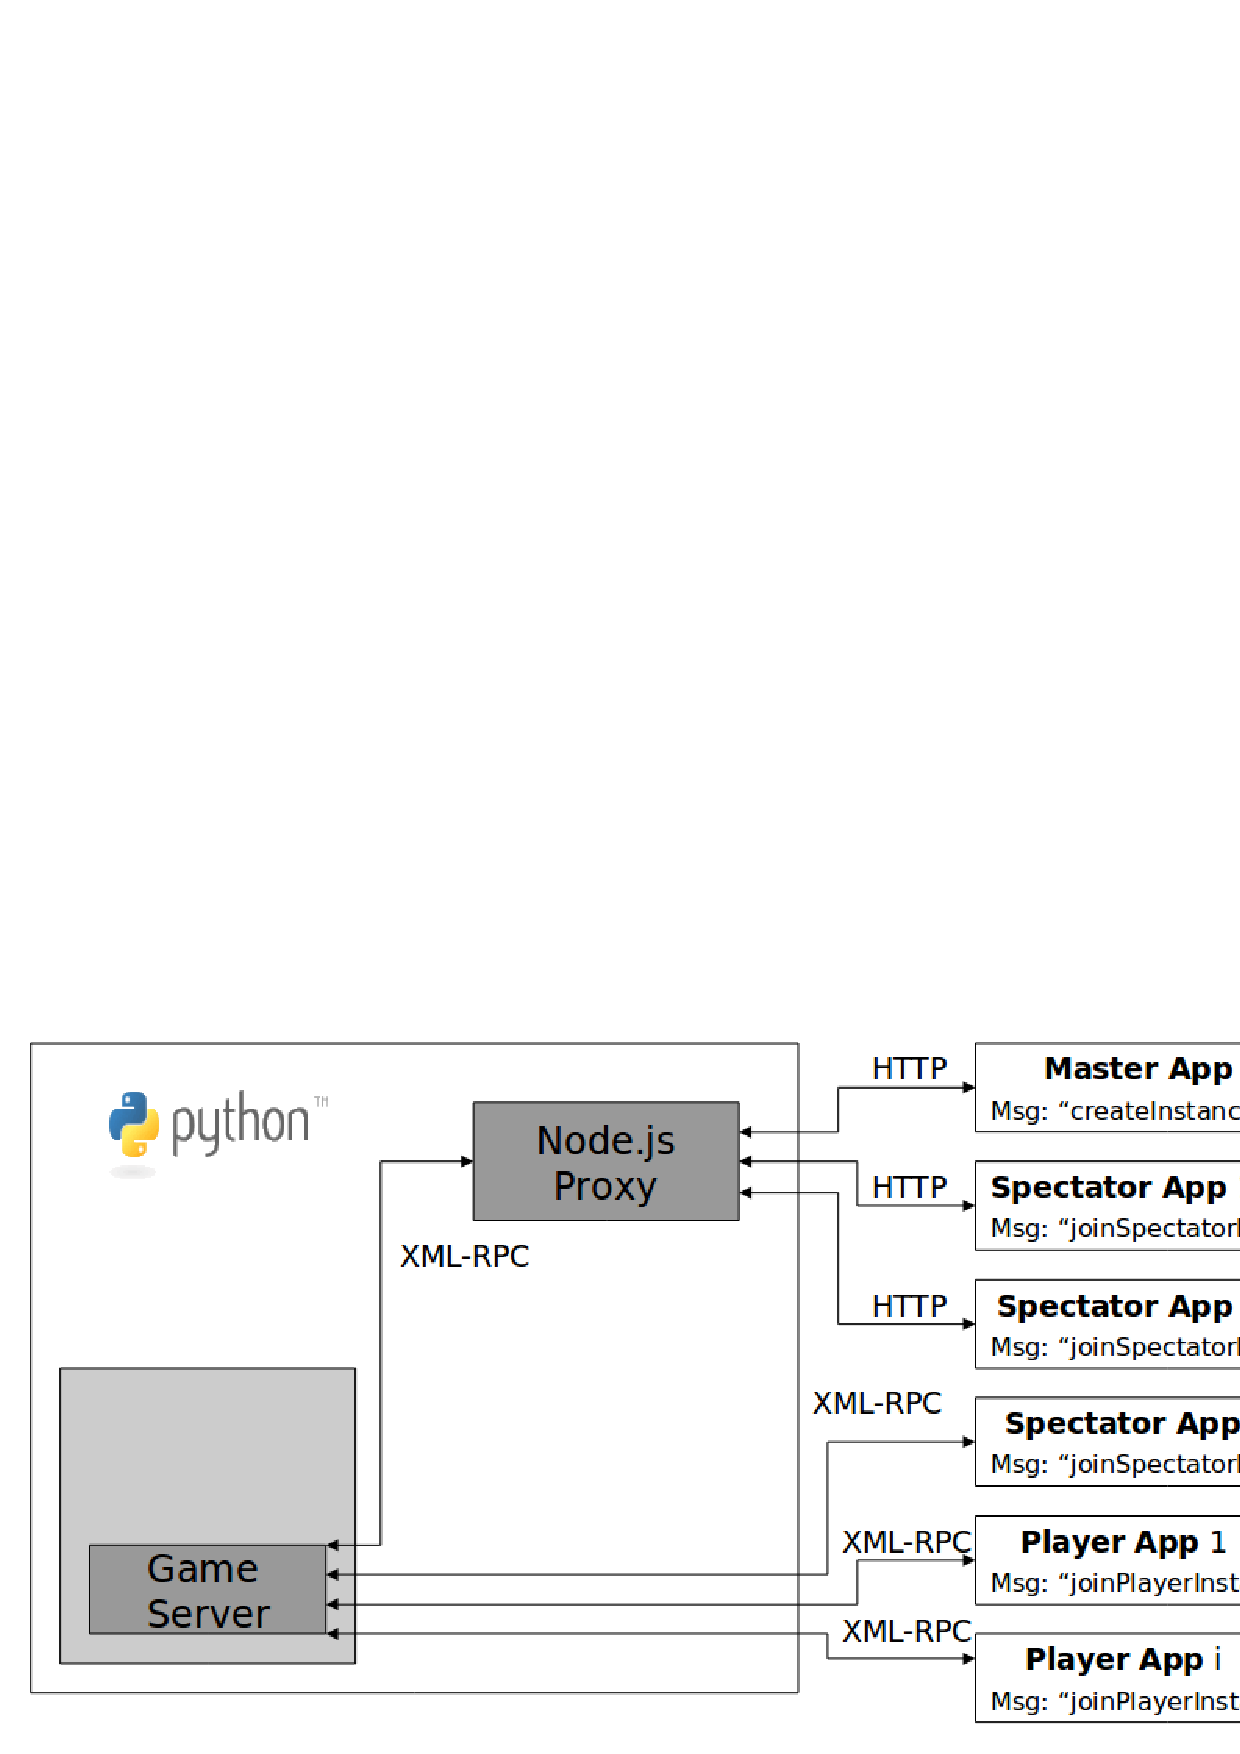
\includegraphics[scale=0.6]{Figures/_step1_xmlrpc}
\caption{System architecture with a focus on the login phase using XML-RPC}
\label{F_step1_xmlrpc}
\end{center}
\end{figure}


\begin{figure}[htbp!]
\begin{center}
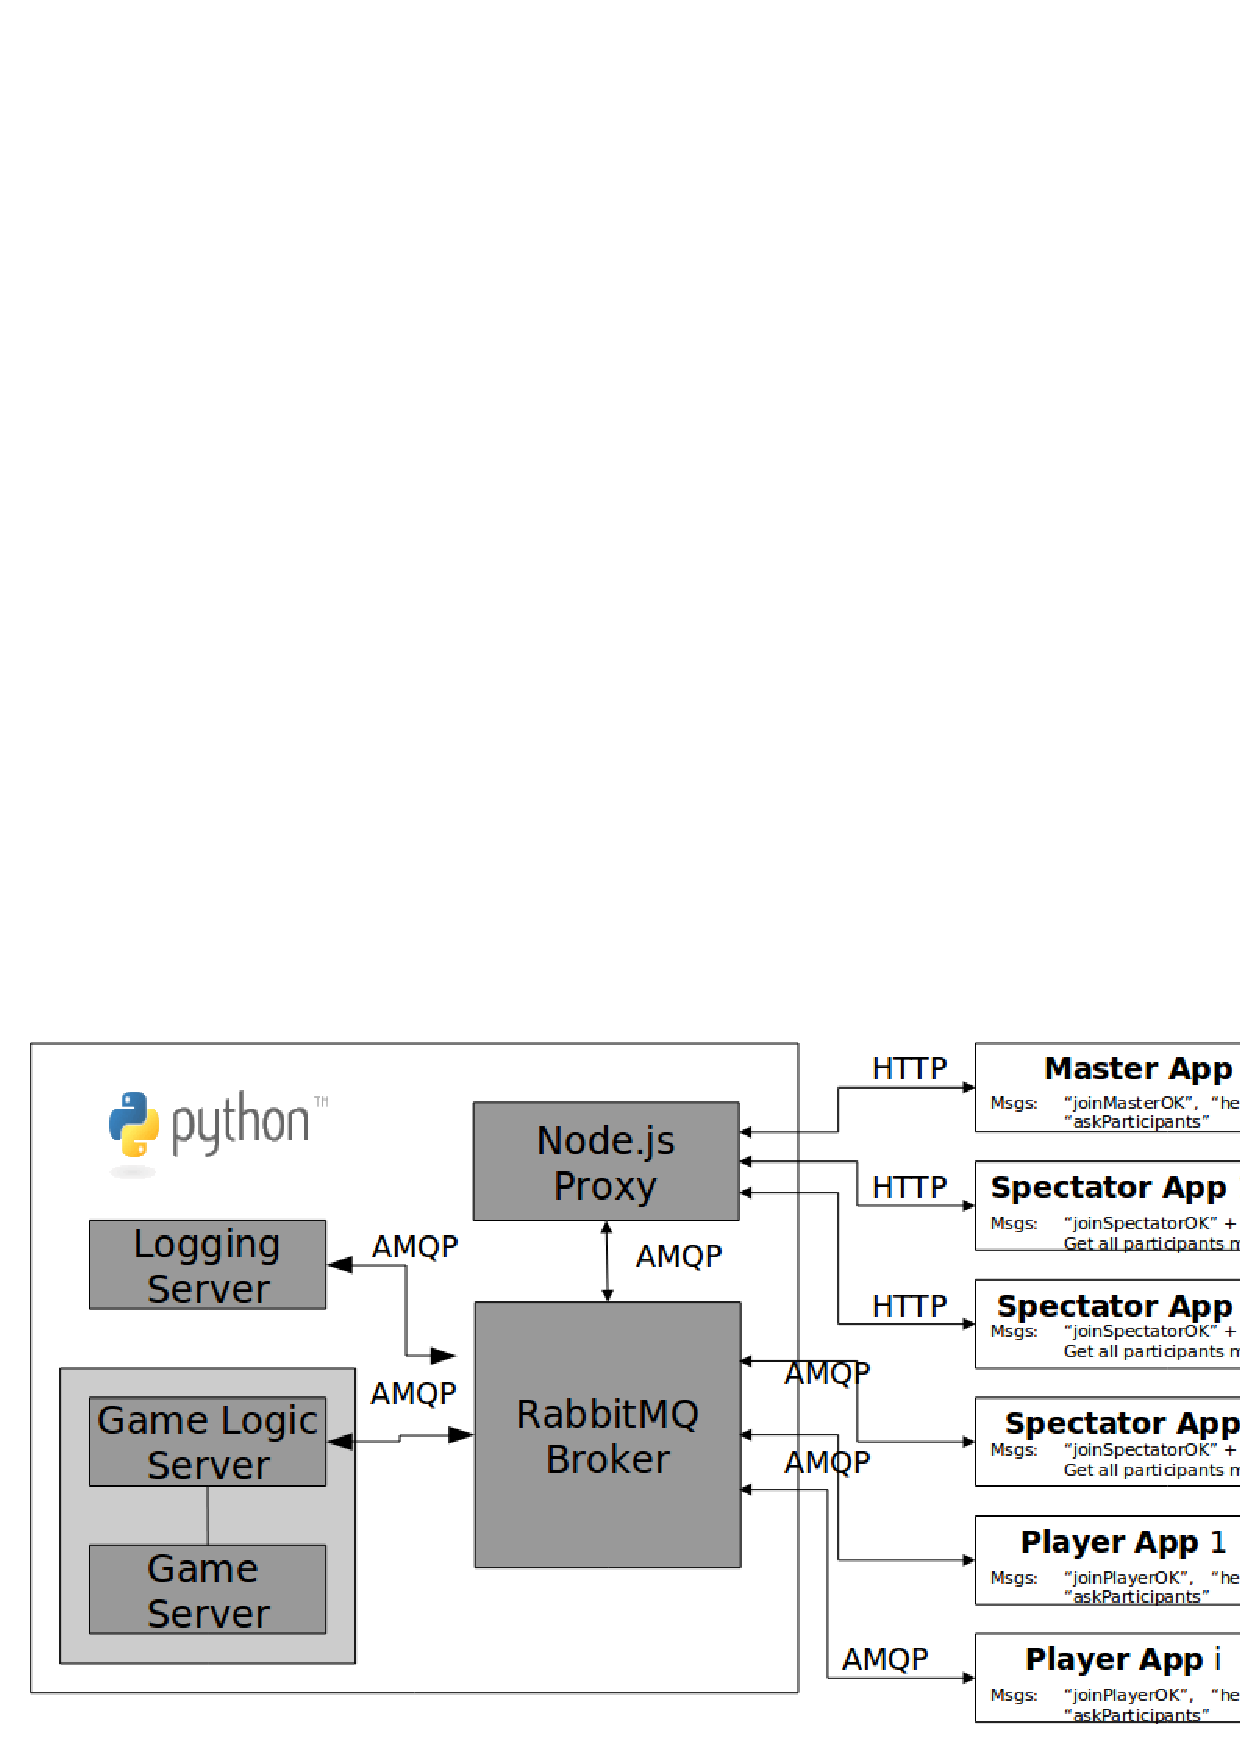
\includegraphics[scale=0.6]{Figures/_step2_amqp}
\caption{System architecture with a focus on the exchanging of messages using 
AMQP}
\label{F_step2_amqp}
\end{center}
\end{figure}

\endinput
